\begin{figure}[b]
    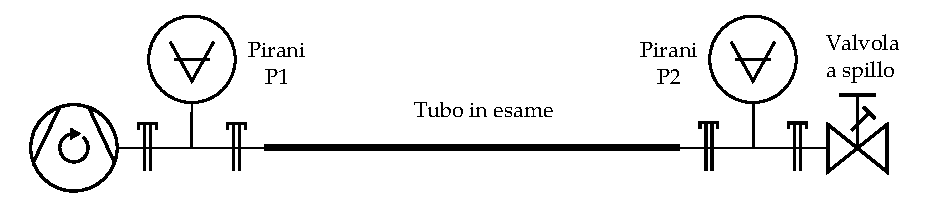
\includegraphics[width=160mm]{drawing.pdf}
    \caption{Schema dell'impianto da vuoto.}
    \label{fig:schema}
\end{figure}

\section{Esecuzione}

L'impianto realizzato è schematizzato in figura \ref{fig:schema}. I vacuometri pirani sono stati disposti
immediatamente ai capi del tubo. Indicheremo le pressioni ai due capi come $P1$ e $P2$, come riportato in figura.
La valvola a spillo è stata collocata in fondo all'impianto. È stata mantenuta
aperta la valvola ausiliaria della stessa al fine di evitare problemi con i volumi morti. 

Dopo aver montato l'impianto abbiamo avviato la pompa rotativa, e aspettato di raggiungere il vuoto limite all'interno
del tubo. Per fare ciò abbiamo monitorato al PC l'andamento della pressione al capo $P2$, assicurandoci che la pressione
si fosse stabilizzata prima di aprire la valvola micrometrica.

Una volta raggiunta la pressione limite abbiamo aperto la valvola micrometrica ad un valore per il quale ci fosse noto
il flusso in entrata. La valvola a spillo è stata tarata nelle esperienze precedenti. A questo punto abbiamo di nuovo
atteso che la pressione si stabilizzasse, prima di misurare la pressione ai capi. 

La procedura è stata ripetuta per 0, 4, 5, 6, 7, 8 giri di apertura della valvola a spillo per ciascuno dei
tubi in esame. Inoltre, per ogni tubo, abbiamo misurato le pressioni aumentando man mano l'apertura della valvola
a spillo per poi misurarle nuovamente chiudendola fino a tornare al valore iniziale.

Durante la sessione di laboratorio abbiamo registrato delle condizioni atmosferiche stabili: $P\ped{atm} = 981 \pm 1$ hPa,
$T = 296 \pm 1 \si{\kelvin}$. Entrambe le misure riportano incertezze di risoluzione.

\section{Analisi dati}


